\section{近似采样下的梯度}
\label{sec:pgrad-approx}

前面的无偏结论都假设样本精确服从$P_{\bm{\theta}}$。实际上，样本常常来自近似的生成器，或来自运行了有限步的Markov链。梯度公式本身是对的，用的样本却不对，结果算的是什么？

\paragraph{三个量}

设梯度公式$\bm{G}=\bm{\phi}_{\bm{\theta}}(X)$在目标下正确，即它在$X\sim P_{\bm{\theta}}$时的期望等于$\nabla J(\bm{\theta})$，而实际样本服从另一个分布$\widetilde{P}_{\bm{\theta}}$。要区分三个量：目标期望的梯度$\nabla J(\bm{\theta})$；公式在实际抽样规律下的均值
\[
  \bar{\bm{g}}(\bm{\theta})=\mathbb{E}_{\widetilde{P}_{\bm{\theta}}}[\bm{\phi}_{\bm{\theta}}(X)];
\]
以及$n$个样本平均$\hat{\bm{g}}_{n}$的有限样本波动。估计误差相应地分成两部分，
\begin{equation}
  \hat{\bm{g}}_{n}-\nabla J(\bm{\theta})=\underbrace{\bigl(\bar{\bm{g}}(\bm{\theta})-\nabla J(\bm{\theta})\bigr)}_{\text{采样偏差}}+\underbrace{\bigl(\hat{\bm{g}}_{n}-\bar{\bm{g}}(\bm{\theta})\bigr)}_{\text{有限样本波动}}.
  \label{eq:pgrad-error-split}
\end{equation}
这和第~\ref{chap:monte-carlo-integration-error}章对积分误差的分解完全相同，因为梯度估计本来就是一个积分估计。

第一部分与样本数无关，增加同一近似方法的样本数不能消除它。若$\bm{\phi}_{\bm{\theta}}$的分量有界，它可以用$\widetilde{P}_{\bm{\theta}}$与$P_{\bm{\theta}}$的总变差距离控制：对取值于$[m_{j},M_{j}]$的分量，偏差的绝对值不超过$(M_{j}-m_{j})\,d_{\mathrm{TV}}(\widetilde{P}_{\bm{\theta}},P_{\bm{\theta}})$。但梯度公式往往无界，例如得分估计里的$f\cdot s$，这时还需要尾部或矩的控制，分布在总变差下接近并不保证期望接近。第二部分取决于样本之间的关系：独立样本时它的方差是单样本方差除以$n$；样本是链上的连续状态时，要用第~\ref{chap:monte-carlo-integration-error}章的长期方差代替单样本方差，相关性可以使误差成倍增大。

\paragraph{一个可以算到底的链}

取目标$\mathcal{N}(\theta,1)$，$f(x)=x^{2}$，$J'(\theta)=2\theta$。用如下的链近似采样：
\[
  X^{(t+1)}=\rho X^{(t)}+(1-\rho)\theta+\sqrt{1-\rho^{2}}\,\varepsilon_{t},\qquad X^{(0)}=0,
\]
$\varepsilon_{t}$独立同分布于$\mathcal{N}(0,1)$，$0<\rho<1$。若$X^{(t)}\sim\mathcal{N}(\theta,1)$，则$X^{(t+1)}$的均值为$\rho\theta+(1-\rho)\theta=\theta$，方差为$\rho^{2}+1-\rho^{2}=1$，所以目标是这条链的不变分布。从$X^{(0)}=0$出发，均值与方差满足
\[
  m_{t+1}=\rho m_{t}+(1-\rho)\theta,\qquad v_{t+1}=\rho^{2}v_{t}+1-\rho^{2},
\]
解出第$K$步$X^{(K)}\sim\mathcal{N}(m_{K},v_{K})$，其中
\begin{equation}
  m_{K}=\theta(1-\rho^{K}),\qquad v_{K}=1-\rho^{2K}.
  \label{eq:pgrad-ar-law}
\end{equation}

把目标下正确的两个公式用在$X^{(K)}$上。重参数化公式$2X$的均值是$2m_{K}=2\theta(1-\rho^{K})$；得分公式$X^{2}(X-\theta)$的均值是
\[
  \mathbb{E}\bigl[(X^{(K)})^{3}\bigr]-\theta\,\mathbb{E}\bigl[(X^{(K)})^{2}\bigr]=m_{K}^{3}+3m_{K}v_{K}-\theta(m_{K}^{2}+v_{K}).
\]
取$\theta=1$、$\rho=0.8$、$K=5$，$\rho^{5}=0.32768$，于是$m_{5}=0.6723$，$v_{5}=0.8926$。两个公式的均值分别为
\[
  2m_{5}=1.345,\qquad m_{5}^{3}+3m_{5}v_{5}-(m_{5}^{2}+v_{5})=0.760,
\]
目标是$2$。同一组近似样本上，两个在目标下都无偏的公式偏差不同，偏差的大小取决于公式本身。

\paragraph{对有限步程序求导}

另一种做法是把整个采样程序当成生成映射，对它做重参数化。展开递推，$X^{(K)}$是$\theta$的仿射函数加上与$\theta$无关的噪声，$\partial X^{(K)}/\partial\theta=1-\rho^{K}$，路径导数为$2X^{(K)}(1-\rho^{K})$。这里每一步都合法：噪声分布固定，函数光滑，交换条件也容易验证。它的期望是程序所定义的期望
\[
  J_{K}(\theta)=\mathbb{E}\bigl[(X^{(K)})^{2}\bigr]=\theta^{2}(1-\rho^{K})^{2}+1-\rho^{2K}
\]
的导数$J_{K}'(\theta)=2\theta(1-\rho^{K})^{2}$，在上面的参数下等于$0.904$，而不是$J'(1)=2$。

也就是说，对有限步采样程序求导并交换积分，得到的是程序期望$J_{K}$的导数；它是否等于目标期望$J$的导数，是另一个需要证明的命题。本例中$J_{K}$对$\theta$的依赖还包含初值$X^{(0)}=0$不随$\theta$移动这一人为因素，所以$J_{K}'$比两个“目标公式”偏得更多。图~\ref{fig:pgrad-chain-bias}画出了三个量随步数$K$的变化，图~\ref{fig:pgrad-error-split}在$K=5$处把式~\eqref{eq:pgrad-error-split}的两部分和程序导数放在一条数轴上比较。

\begin{BookInlineFigure}
  \centering
  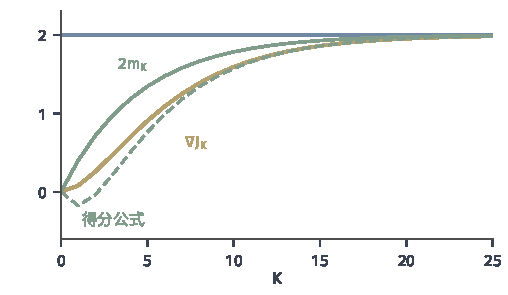
\includegraphics[width=86mm]{figures/07-probability/08-sampling-and-integration/matplotlib/pgrad-chain-bias/figure.pdf}
  \caption{目标$\mathcal{N}(1,1)$、$f(x)=x^{2}$，样本取自从$0$出发、$\rho=0.8$的链的第$K$步。蓝线为目标梯度$2$；绿实线为重参数化公式$2X$在第$K$步分布下的均值$2m_{K}$；绿虚线为得分公式$X^{2}(X-1)$在同一分布下的均值；黄线为有限步程序期望的导数$J_{K}'$。}
  \label{fig:pgrad-chain-bias}
\end{BookInlineFigure}

\begin{BookInlineFigure}
  \centering
  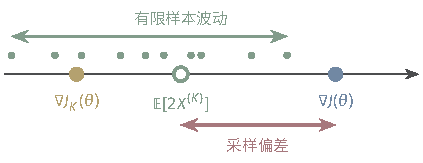
\includegraphics[width=72mm]{figures/07-probability/08-sampling-and-integration/tikz/pgrad-error-split/figure.pdf}
  \caption{图~\ref{fig:pgrad-chain-bias}中$K=5$时的误差分解。蓝点为目标梯度$\nabla J(1)=2$；绿圈为公式$2X$在实际抽样规律下的均值$1.345$，它与蓝点之差是采样偏差；上方绿点为$10$次独立重复中$n=20$个样本平均的取值（固定种子），其散布是有限样本波动；黄点为有限步程序的导数$0.904$。}
  \label{fig:pgrad-error-split}
\end{BookInlineFigure}

\paragraph{步数增加时}

本例中$K\to\infty$时三个量都趋于$2$，因为式~\eqref{eq:pgrad-ar-law}给出了闭式。一般情形下，即使$J_{K}\to J$，也推不出$J_{K}'\to J'$。例如
\[
  J_{K}(\theta)=J(\theta)+\frac{1}{K}\sin(K\theta)
\]
满足$\lvert J_{K}-J\rvert\leq1/K$，但$J_{K}'-J'=\cos(K\theta)$不趋于零。函数值的一致逼近不控制导数。要由程序导数得到目标导数，需要导数本身的收敛，例如$J_{K}'$在$\theta$的某个邻域上一致收敛，这时微积分中关于导数一致收敛的定理保证极限就是$J'$。对实际的MCMC程序，这类结论要用到链对参数的可微依赖与遍历性的定量估计，超出了本卷给定分布计算的范围。

实际计算时，比较稳妥的做法是：用前几节在目标下成立的梯度公式，把链上的样本当作计算这个期望的积分样本，然后按第~\ref{chap:monte-carlo-integration-error}章检查初值偏差、相关性与长期方差。这样，梯度的正确性来自目标下的公式，误差的分析来自积分误差的理论，两者各有依据。
